\chapter{Model Integration and Analysis Framework}
\label{chap:model-integration-and-analysis-framework}

Accurate flood risk assessment requires the integration of diverse data sources and computational tools to simulate hazard intensity, estimate potential damages, and evaluate financial exposure. In this chapter, we present the technical framework developed to combine heterogeneous flood hazard data—particularly local Slovenian models—into a unified system suitable for analysis and comparison within the Physrisk platform.

The focus lies on harmonizing the \textit{Integralna karta globin} (IKG) flood maps, which vary in structure, format, and coordinate reference systems, and transforming them into a consistent, machine-readable representation. These models are rasterized, standardized by return period, and encoded in the cloud-optimized Zarr format. The processed datasets are then onboarded into the modular Physrisk platform, which separates hazard, vulnerability, and financial components and allows for flexible model evaluation.

To facilitate empirical comparison, the framework also includes a toolset that enables side-by-side querying and batch evaluation of both global and local models at precise geolocations, aligned with the validation dataset. This infrastructure supports all subsequent experimental analysis presented in Chapter~\ref{chap:experimental-analysis} and lays the groundwork for scalable, reproducible physical climate risk assessments.

The chapter is organized as follows:
\begin{itemize}
    \item Section~4.1 presents the overall system architecture and the interaction between components.
    \item Section~4.2 describes the pipeline for transforming and combining IKG models across multiple areas of significant importance.
    \item Section~4.3 explains how the standardized hazard data are integrated into the Physrisk platform.
    \item Section~4.4 outlines the model comparison toolset used to evaluate prediction accuracy across models.
\end{itemize}

\section{Architectural Diagram}

The integration of global and local flood hazard models into a unified analysis platform requires a modular, extensible architecture that supports heterogeneous input formats, scenario-aware modeling, and scalable evaluation. This section presents the architecture developed for this purpose, highlighting its components, data flow, and interoperability within the \textit{Physrisk} framework.

\subsection{System Overview}

Figure~\ref{fig:physrisk-overview-components} illustrates the architecture of the flood hazard model integration pipeline, based on the open-source \textit{OS-Climate Physrisk} ecosystem. The process begins with raw flood hazard data, which may originate from global sources such as the WRI Aqueduct or TU Delft flood models, or from local sources such as the Integralna karta globin (IKG) used in Slovenia. These datasets are onboarded into the \texttt{os-risk-hazard} module, a Python-based processing library designed to standardize, harmonize, and prepare hazard indicators for risk evaluation.

The onboarded models are then encoded in Zarr format and stored in an AWS S3-compatible object storage. The Physrisk framework retrieves hazard indicators from this backend and combines them with vulnerability and exposure components to compute impact distributions. The resulting outputs can be accessed via the Physrisk API or used directly for ESG reporting and financial risk analysis through the \texttt{os-risk-financial} module.

\begin{figure}[htb]
    \centering
    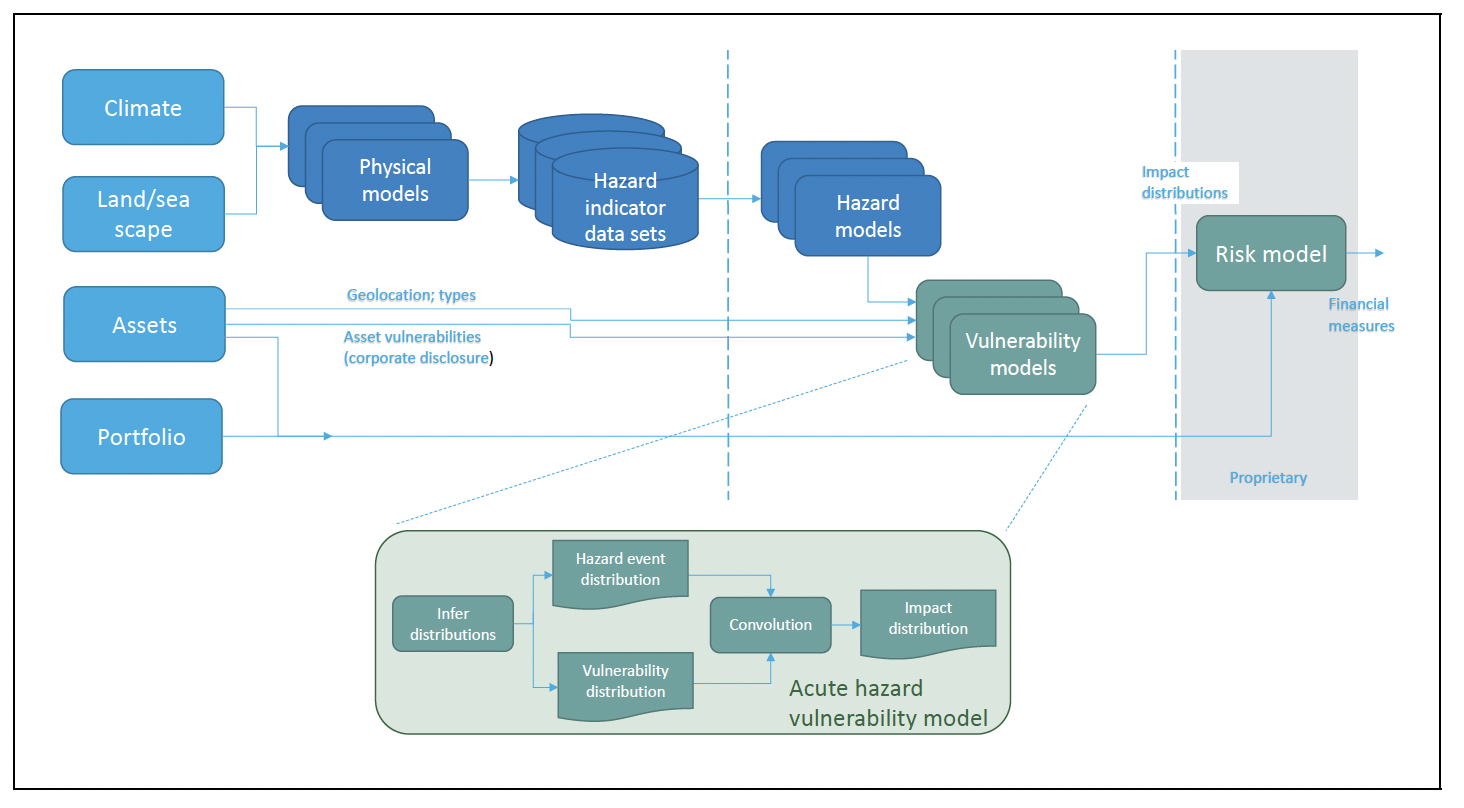
\includegraphics[width=0.9\textwidth]{figures/04/physrisk-overview-components.png}
    \caption[Physrisk physical risk model components.]{Conceptual architecture of a physical climate risk model, showing the integration of hazard data, vulnerability models, and asset-level exposure to produce impact distributions. Adapted from the CVAR Physrisk methodology \cite{moorhouse2024}.}
    \label{fig:physrisk-overview-components}
\end{figure}


\subsection{Data Flow and Model Interoperability}

Each flood model—whether global or local—is processed through the same onboarding interface, allowing standardization of outputs while preserving return-period-specific intensity information. The hazard models are structured into three-dimensional Zarr arrays indexed by latitude, longitude, and return period. This enables consistent querying and evaluation across models with different spatial resolutions or geographic coverage.

Once onboarded, all hazard layers become interchangeable within the Physrisk pipeline. Vulnerability models (e.g., depth--damage functions) and exposure datasets (e.g., building values or asset locations) can then be used in combination with any hazard source. This interoperability allows for both comparative experiments and compound risk evaluations, where multiple models are used to bound uncertainty or stress-test assumptions.

\subsection{Integration of the IKG Model}

The locally developed IKG model, originally provided in shapefile and GeoPackage vector formats, required a dedicated pre-processing stage to align with the Physrisk architecture. This process involved:
\begin{itemize}
    \item Transforming coordinate systems (from EPSG:3794 to EPSG:4326),
    \item Rasterizing vector layers into a fixed-resolution 5x5m grid,
    \item Assigning discrete flood depth values to each return period (RP10, RP100, RP500),
    \item Converting the raster layers into Zarr format for chunked cloud storage.
\end{itemize}

The unified model was then uploaded to AWS S3 and integrated into the Physrisk hazard module alongside WRI Aqueduct (and other, already onboarded models). This enabled direct comparison and batch evaluation of global versus local model predictions, described further in Section~\ref{sec:comparison-toolset}.

\begin{figure}[htb]
    \centering
    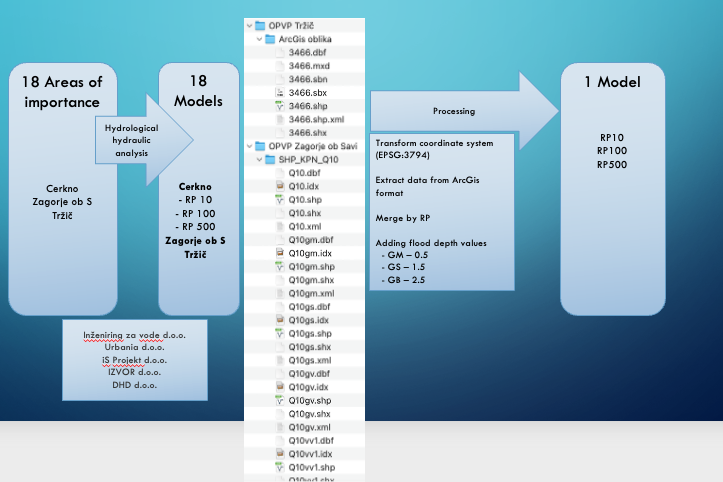
\includegraphics[width=0.95\textwidth]{figures/04/ikg_processing_pipeline.png}
    \caption[Processing heterogeneous IKG flood models.]{Pipeline for combining flood hazard data from 18 distinct Slovenian municipalities. Each area includes return-period-specific vector layers (e.g., shapefiles), which are transformed, reprojected, assigned standardized flood depth values (0.5 m, 1.5 m, 2.5 m), and merged into a single harmonized hazard model.}
    \label{fig:ikg_processing_pipeline}
\end{figure}

\subsection{Hazard Onboarding Pipeline}

The transformation from raw IKG data into a cloud-optimized flood hazard model is summarized in Figure~\ref{fig:ikg_physrisk_onboarding_pipeline}. The pipeline consists of the following steps:
\begin{enumerate}
    \item \textbf{Rasterization:} Converting input vector data into gridded raster tiles using a 5x5m resolution grid.
    \item \textbf{Zarrify:} Chunking the raster into 1000x1000 tiles and encoding into Zarr format.
    \item \textbf{Upload:} Transferring the data to AWS S3 for use within Physrisk.
\end{enumerate}

The final onboarded dataset can be queried via the Physrisk API or accessed directly for integration with ESG tools or batch model evaluation.

\begin{figure}[htb]
    \centering
    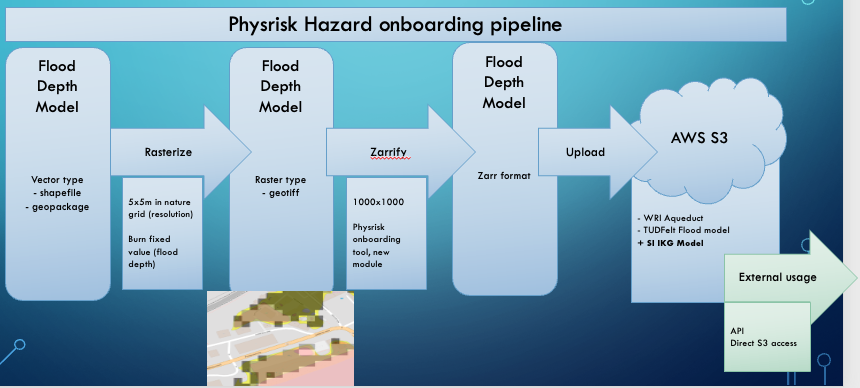
\includegraphics[width=0.9\textwidth]{figures/04/ikg_physrisk_onboarding_pipeline.png}
    \caption[Physrisk hazard onboarding pipeline.]{The onboarding pipeline for flood depth models into Physrisk. The process begins with vector data (e.g., shapefiles), rasterizes them into a 5x5 m resolution grid, converts to cloud-optimized Zarr format using the Physrisk onboarding tool, and uploads to AWS S3 for programmatic use.}
    \label{fig:ikg_physrisk_onboarding_pipeline}
\end{figure}

\section{Pipeline for Combining Heterogeneous IKG Models}

The \textit{Integralna karta globin} (IKG) flood hazard datasets are developed for individual municipalities or regions in Slovenia, each based on local hydrological and hydraulic analyses. These datasets differ in file structure, geospatial reference systems, data quality, and encoding of flood depths. To integrate these into a unified flood hazard model suitable for comparative evaluation and platform onboarding, a standardized processing pipeline was developed.

\subsection{Data Sources and Heterogeneity}

The raw IKG datasets were obtained from multiple engineering consultancies (\textit{Inženiring za vode d.o.o., Urbania d.o.o., iS Projekt d.o.o., IZVOR d.o.o., DHD d.o.o.}), each responsible for flood modeling in a subset of areas classified as "Območja pomembnega vpliva" (Areas of Significant Flood Risk) by Slovenian water authorities.

Each local model typically includes:
\begin{itemize}
    \item GIS vector data (shapefiles, GeoPackages) representing inundation zones,
    \item Attribute data encoding flood extent and classes for selected return periods (e.g., 10-, 100-, and 500-year events),
    \item Region-specific coordinate systems (typically EPSG:3794, Slovenia National Grid).
\end{itemize}

In total, data from 18 areas of importance were collected, with each area providing flood scenarios for three return periods. This resulted in 54 distinct layers that needed to be harmonized.

\subsection{Standardization and Processing Workflow}

To unify the IKG datasets into a single model, the following pipeline was developed and implemented in Python using open-source geospatial processing libraries (GDAL, Fiona, Rasterio, xarray):

\begin{enumerate}
    \item \textbf{Coordinate Transformation:} All source files were transformed from EPSG:3794 to WGS84 (EPSG:4326) to ensure compatibility with global models and standardized grid alignment.
    
    \item \textbf{Rasterization:} Vector layers were rasterized into a regular grid with a resolution of 5 meters (5x5m), which approximates the native resolution of the original hydrological models. A fixed flood depth value was assigned to each flood class:
    \begin{itemize}
        \item GM (minor flooding): 0.5 m
        \item GS (significant flooding): 1.5 m
        \item GB (severe flooding): 2.5 m
    \end{itemize}
    
    \item \textbf{Return Period Alignment:} Each rasterized layer was tagged with its associated return period (RP10, RP100, RP500). For each area, three separate rasters were produced and stacked by return period.
    
    \item \textbf{Tiling and Merging:} The processed rasters from all areas were mosaicked into a common spatial grid and stored as a 3D array indexed by latitude, longitude, and return period. Conflicts in overlapping regions (e.g., model boundaries) were resolved by assigning priority to higher-confidence datasets based on metadata quality.
\end{enumerate}

\subsection{Unified Flood Hazard Product}

The final result of this pipeline is a unified flood hazard model for Slovenia covering all 18 areas of importance for the 3 defined return periods. This model:
\begin{itemize}
    \item Captures flood depth estimates at high spatial resolution for three return periods,
    \item Standardizes input data from diverse local models into a single harmonized format,
    \item Enables consistent comparison with global models such as WRI Aqueduct within the same framework.
\end{itemize}

Figure~\ref{fig:ikg_processing_pipeline} provides a schematic representation of the transformation process, from raw shapefiles to a standardized hazard product.

This unified model was subsequently converted to Zarr format and onboarded into the Physrisk platform, as described in Section~\ref{sec:physrisk-framework-model-onboarding}.


%--------------------------------------------------------------------------------------------------
\section{Physrisk Framework – Model Onboarding}
\label{sec:physrisk-framework-model-onboarding}
%--------------------------------------------------------------------------------------------------

Once the local IKG flood models were unified into a standardized and spatially consistent format, the next step involved integrating them into the modular \textit{Physrisk} framework. Physrisk is part of the broader OS-Climate open-source ecosystem and is designed to facilitate scalable, scenario-based physical climate risk analysis. The framework separates hazard, vulnerability, and financial components and enables flexible model composition, comparison, and evaluation.

\subsection{Physrisk Architecture and Modules}

The Physrisk architecture is composed of several interoperable modules:

\begin{itemize}
    \item \textbf{OS-risk-hazard}: responsible for ingesting and formatting hazard data sets (e.g., flood depth by return period) into a common format.
    \item \textbf{OS-risk-physrisk}: computes impact distributions by convolving hazard data with vulnerability functions and exposure information.
    \item \textbf{OS-risk-financial}: translates physical impacts into financial metrics such as loss of asset value or disruption to operations.
    \item \textbf{Physrisk API}: exposes model outputs through a standardized programmatic interface.
\end{itemize}

The onboarding of hazard models occurs within the \texttt{os-risk-hazard} component and requires the hazard data to conform to a Zarr-based storage structure optimized for parallel access and spatial querying.

\subsection{Zarr Format and Indexing}

The Zarr format is a cloud-native format for storing large multi-dimensional arrays. It was chosen for hazard model storage due to its ability to:
\begin{itemize}
    \item Efficiently compress and store gridded data in chunks (e.g., 1000×1000 tiles),
    \item Allow selective download of spatial subsets,
    \item Support multi-indexing (e.g., latitude, longitude, return period).
\end{itemize}

For the unified IKG model, the hazard data were encoded into a 3-dimensional Zarr array with the following dimensions:
\begin{itemize}
    \item $i$: Latitude (y-axis),
    \item $j$: Longitude (x-axis),
    \item $k$: Return period index, corresponding to RP10, RP100, and RP500.
\end{itemize}

Each tile was stored as a compressed chunk and uploaded to an AWS S3-compatible bucket accessible to all Physrisk modules.

\subsection{Onboarding Procedure}

The onboarding process was implemented using the Physrisk hazard onboarding tool, a Python-based utility designed for structured hazard model integration. The steps were as follows:

\begin{enumerate}
    \item \textbf{Prepare Metadata:} Define the return periods, CRS (EPSG:4326), spatial resolution, and transformation matrix for the IKG model.
    
    \item \textbf{Convert to Zarr:} Use the onboarding tool to encode the processed GeoTIFF files into a Zarr store, assigning appropriate chunk sizes (e.g., 1000×1000 pixels).
    
    \item \textbf{Upload to Cloud Storage:} Transfer the Zarr directory to a cloud-accessible S3 bucket used by the OS-Climate infrastructure.
    
    \item \textbf{Register the Model:} Add a model reference entry into the hazard configuration of Physrisk, enabling downstream access via API and batch processors.
\end{enumerate}

\subsection{Integration with Other Models}

With the IKG model onboarded, it became available in the same infrastructure alongside global flood hazard layers, including:
\begin{itemize}
    \item WRI Aqueduct River Flood (global, ~1 km resolution),
    \item TU Delft River Flood (Pan-European, ~100 m resolution).
\end{itemize}

This interoperability allows any of the onboarded hazard layers to be used with common vulnerability functions and exposure datasets, enabling direct comparisons, uncertainty bounding, and ensemble evaluations. The IKG model is now fully accessible via the Physrisk API and can be used for property-level flood risk analysis in Slovenia under a unified modeling interface.

%--------------------------------------------------------------------------------------------------
\section{Comparison Toolset}
\label{sec:comparison-toolset}
%--------------------------------------------------------------------------------------------------

To evaluate and compare the predictive performance of flood hazard models, a model-agnostic comparison toolset was developed and integrated into the Physrisk framework. This toolset enables side-by-side querying of multiple hazard sources at specific geolocations and return periods, aligned with the reference flood observations used for validation in Chapter~5.

\subsection{Purpose and Design Principles}

The comparison toolset was designed with the following goals in mind:
\begin{itemize}
    \item \textbf{Model-agnostic access:} Allow querying of different onboarded hazard models (e.g., IKG, WRI Aqueduct) through a unified interface.
    \item \textbf{Return-period specificity:} Ensure comparability by extracting flood depth predictions at the same return period (e.g., 100-year flood).
    \item \textbf{Location-accurate evaluation:} Retrieve model outputs at high spatial precision to match reported flood locations.
    \item \textbf{Batch processing support:} Enable evaluation across hundreds of observations using efficient geospatial access patterns.
\end{itemize}

\subsection{Interface and Functionality}

The toolset consists of a lightweight Python interface built on top of the Physrisk hazard API. Given a set of coordinates (latitude, longitude) and a desired return period, the tool performs the following steps:

\begin{enumerate}
    \item \textbf{Coordinate Transformation:} Convert input coordinates into the grid index of the onboarded Zarr array using affine transformations defined in the model metadata.
    
    \item \textbf{Chunk Identification and Retrieval:} Locate the Zarr chunk containing the requested point and load the corresponding depth value for the specified return period.
    
    \item \textbf{Output Formatting:} Return the flood depth value, return period, and model metadata for downstream use in regression or classification analysis.
\end{enumerate}

When applied in batch mode, the tool leverages parallel reads and lazy loading to evaluate large datasets (e.g., the full validation set of flood reports) with minimal memory overhead.

\subsection{Supported Models and Inputs}

The toolset was validated for use with the following onboarded hazard models:

\begin{itemize}
    \item \textbf{SI IKG (Unified Model)}: High-resolution local flood model rasterized at 5x5 m, covering 18 Slovenian areas of importance, with RP10, RP100, and RP500 layers.
    \item \textbf{WRI Aqueduct Flood Hazard}: Global model with ~1 km resolution, scenario-aware, supporting multiple return periods from RP2 to RP1000.
\end{itemize}

The input to the toolset is a tabular dataset containing:
\begin{itemize}
    \item Latitude and longitude of each observation,
    \item Desired return period (e.g., RP100),
    \item Optional fields: timestamp, municipality, reported depth, reported damage.
\end{itemize}

\subsection{Integration with Validation Workflow}

The comparison outputs are stored in a structured table, allowing for direct computation of model performance metrics such as:
\begin{itemize}
    \item \textbf{Regression error:} difference between predicted and observed flood depths,
    \item \textbf{Classification accuracy:} match rate within flood depth categories (e.g., $<$0.5 m, 0.5–1.5 m, $>$1.5 m),
    \item \textbf{Bias analysis:} mean and median error segmented by proximity to water, terrain type, or municipality.
\end{itemize}

These outputs form the quantitative basis for the experimental results presented in Chapter~5.

\subsection{Reproducibility and Extensibility}

The toolset was developed as a standalone module and version-controlled as part of the project’s repository. This design ensures that future updates to hazard models (e.g., inclusion of climate scenario variants or additional regions) can be incorporated without changes to the validation logic.

Furthermore, the modularity of the toolset supports extension to:
\begin{itemize}
    \item Additional hazard types (e.g., pluvial flooding),
    \item Vulnerability assessments (via model chaining),
    \item Scenario-based risk projections (by switching hazard layers).
\end{itemize}

Thus, the comparison toolset serves not only as a core utility for this thesis, but also as a scalable evaluation framework for broader applications in physical climate risk modeling.
